\documentclass[12pt,letterpaper]{article}
\usepackage{cite}
\usepackage{amsmath}
\usepackage{amsfonts}
\usepackage{array}
\usepackage{dsfont}
\usepackage{amssymb}
\usepackage{amsthm}
\usepackage{bbold}
\usepackage{fullpage}
\usepackage{mathtools}
\usepackage{enumitem}
\usepackage{mathrsfs}
\usepackage[margin=0.9 in]{geometry}
\usepackage{hyperref}
\usepackage{graphicx}
\usepackage{gensymb}
\usepackage{xcolor,colortbl}
\usepackage[format=plain,
labelfont={bf,it},
textfont={it}]{caption}
\usepackage{float}


\newcommand*{\SignatureAndDate}[1]{%
	\par\noindent\makebox[2.5in]{\hrulefill} \hfill\makebox[2.0in]{\hrulefill}%
	\par\noindent\makebox[2.5in][l]{#1}      \hfill\makebox[2.0in][l]{Date}%
}%
\newcolumntype{L}{>{\centering\arraybackslash}m{2cm}}
\newcolumntype{P}{>{\centering\arraybackslash}m{3cm}}
\newcolumntype{Q}{>{\centering\arraybackslash}m{4cm}}
\setlength{\parindent}{0em}

\allowdisplaybreaks

\newcommand{\R}{\mathds{R}}
\newcommand{\Z}{\mathds{Z}}
\newcommand{\Rplus}{\mathds{R}_{> 0}}
\newcommand{\Zplus}{\mathds{Z}_{\geq 0}}
\newcommand{\F}{\mathds{F}}
\newcommand{\N}{\mathds{N}}
\newcommand{\T}{\mathds{T}}
\newcommand{\s}{\mathds{S}}
\newcommand{\C}{\mathds{C}}
\newcommand{\CDFT}{\mathscr{F}_{CD}} %Fourier transform
\newcommand{\ip}[2]{\langle #1, #2\rangle}


\setlength{\parskip}{0.5em}


\makeatletter
\newsavebox\myboxA
\newsavebox\myboxB
\newlength\mylenA

\begin{document}

\section{Model Development}

\subsection{Core Assumptions}

With the mathematical concepts and software tools clearly defined, a number of assumptions need to be made for the RipStik model.
\par
The RipStik will be treated as 5 separate bodies; the torsion rod (1), front plate (2), back plate (3), front caster (4), and back caster (5).

\begin{figure}[!htb]
	\centering
	\minipage{0.7\textwidth}
	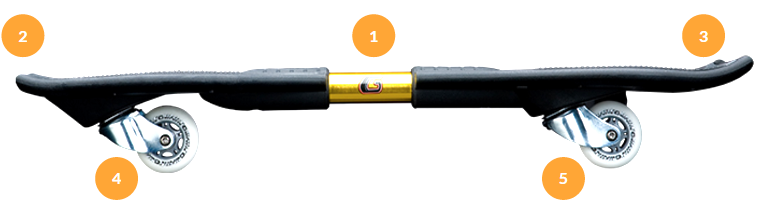
\includegraphics[width=\linewidth]{RipStikModel}
	\caption{Image depicting the 5 separate bodies of the RipStik}\label{fig:RipStikModel}
	\endminipage
\end{figure}  

Difficulties associated with accurately modelling the complex geometry of the RipStik led to simplifying assumptions being made for the shapes of the 5 separate bodies.
The front and back plates were treated as rectangular prisms while defining inertia tensors for the bodies, and the inertia tensors for the wheels were combined with the casters. 
Additionaly, the casters were treated as skates to emulate the constrained motion of the casters while simplifying the overall system dynamics.
\par
The spring in the torsion rod was omitted since it is not a critical component of the RipStik and will add unnecessary complexity to the system in the form of kinetic energy.
Friction between the bodies of the RipStik was omitted, since it would be difficult to accurately model and does not have a significant impact on the general dynamics of the system.
 
\subsection{Coordinate Systems}
The initial focus for developing a mathematical model of the RipStik was placed on determining the number of degrees of freedom in the system. 
A coordinate system was defined, assumptions were made, and Euler angles were applied to said coordinate system so that all degrees of freedom could be explicitly defined.
\par
A body-fixed coordinate system for the RipStik was developed such that the origin was placed at the center of the torsion bar. The X-Y plane will be parallel with the RipStik Deck at rest with no torsion applied.
The +X direction points through the torsion bar towards the front plate, and the Y axis is defined perpendicular to the X axis. The Z axis is normal to the X-Y plane, with +Z pointing upwards. The +Y direction is defined based on the right hand rule.

With the coordinate system defined, Euler angles were implemented into the system to represent the roll ($\alpha$), pitch ($\psi$), and yaw ($\theta$).
\par
The roll angles ($\alpha$) describe the rotation of the deck platform about the X-axis. There will be two roll angles on the RipStik, the first on the front platform ($\alpha_{fp}$) and the second on the rear platform ($\alpha_{bp}$).
\par
The pitch angle ($\psi$) is the angle that the wheels make, offset by the caster angle ($\phi$). This represents a rotation about the Y axis. The wheels are completely unbounded in their ability to rotate, and can pivot through [0, 2$\pi$].
\par
The yaw angle ($\theta$) was represented by a moment taken around the Z-axis (right hand rule applied). There will be two yaw angles on the RipStik, the first on the front caster ($\theta_{fc}$), and the second on the back caster ($\theta_{bc}$).

The RipStik has ten degrees of freedom represented by [X, Y, Z, $\alpha$, $\psi$, $\theta$, $\alpha_{fp}$, $\alpha_{bp}$, $\theta_{fc}$, $\theta_{bc}$].

\subsubsection{Test Case}

In order to validate the selected coordinate system, a test case was conducted for RipStik. This was done by analyzing the behaviour of the caster as it went through a full revolution (2$\pi$ radians).
The output for the X,Y, and Z positions were plotted as a function of the casters rotation as seen in figure \ref{fig:CasterWheel2DTest}.

\begin{figure}[!htb]
	\centering
	\minipage{0.7\textwidth}
	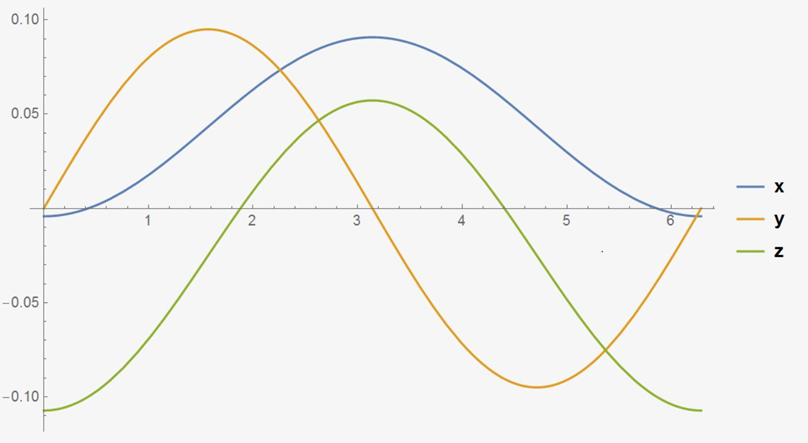
\includegraphics[width=\linewidth]{CasterWheel2DTest}
	\caption{The X ,Y, and Z positions of the caster were plotted as a function of the caster angle (in radians)}\label{fig:CasterWheel2DTest}
	\endminipage
\end{figure} 

With the two-dimensional plot completed, a three-dimensional plot was created to ensure that the casters obeyed the caster orientation that was previously defined, and can be seen in figure \ref{fig:CasterWheel3DTest}.

\begin{figure}[!htb]
	\centering
	\minipage{0.7\textwidth}
	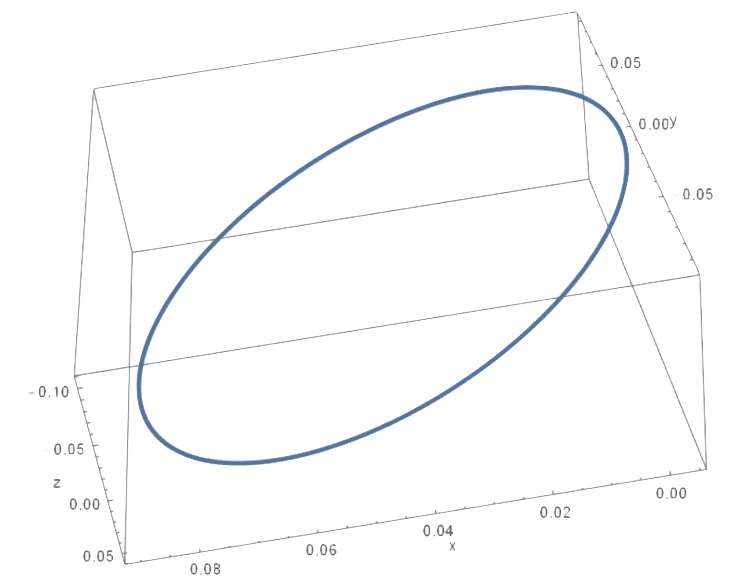
\includegraphics[width=\linewidth]{CasterWheel3DTest}
	\caption{The X ,Y, and Z positions of the caster were plotted as a function of the caster angle (in radians) on a three-dimensional plot}\label{fig:CasterWheel3DTest}
	\endminipage
\end{figure} 

\subsubsection{Model Implementation}
With the test case completed and verified, the coordinate system for the RipStik model was verified for each degree of freedom in the system. 
This was completed by taking applying the output from Mathematica into a visualization software (threejs).

\subsubsection{Validation}
Each degree of freedom in the system behaved as expected. 
Therefore, the selected coordinate system was correct, and the equations of motion can be developed.

\subsection{Equations of Motion}
To develop the equations of motion for the RipStik, the Lagrangian needs to be clearly developed. Given equation \ref{eq:Lagrange}, it is necessary to break down the components of kinetic and potential energies in the system.

The kinetic energy in the system is composed of translational and rotational components.
The Translational Kinetic Energy (TKE) is modeled in the following fashion:

\begin{equation}
\label{eq:TKE}
\text{TKE} = \frac{1}{2}{\text{m}}{\lvert \lvert {\dot{\text{r}}^2} \rvert \rvert}
\end{equation}

In equation \ref{eq:TKE}, m represents the mass of the body and $\dot{r}$ represents the translational velocity of the body.
\par
The Rotational kinetic energy (RKE) is modeled in the following fashion:

\begin{equation}
\label{eq:RKE}
\text{RKE} = \frac{1}{2}({\text{I}}{\omega(t)})^T\omega(t)
\end{equation}

In equation \ref{eq:RKE}, I represents the inertia tensor of the body, and $\omega(t)$ represents the angular velocity of the body.

Finding the angular velocity for the body requires the following process. First, $\hat{\omega(t)}$ is solved for using equation \ref{eq:omegahat}.

\begin{equation}
\label{eq:omegahat}
\hat{\omega}(t)=R^T(t)\dot{R(t)}
\end{equation}

Equation \ref{eq:omegahat} generates a 3x3 skew-symmetric matrix. The angular velocity is then a column vector composed of 3 elements from $\hat{\omega}(t)$, seen in equation \ref{eq:omega}.

\begin{equation}
\label{eq:omega}
\omega(t)=\begin{bmatrix}
\hat{\omega}(t)[3,2] \\
\hat{\omega}(t)[1,3] \\
\hat{\omega}(t)[2,1]\\
\end{bmatrix}
\end{equation}

The potential energy in the system is composed of only Gravitational Potential Energy (GPE). This is modelled by equation \ref{eq:GPE}.

\begin{equation}
\label{eq:GPE}
\text{GPE} = {\text{m}}{\text{g}}{\text{h}}
\end{equation}

In equation \ref{eq:GPE}, m represents the mass of the body and h represents the height of the body relative to the ground plane.

With the kinetic and potential energies explicity defined, the Lagrangian can be written as follows:

\begin{equation}
L= \frac{1}{2}{\text{m}}{\lvert \lvert {\dot{\text{r}}^2} \rvert \rvert} + \frac{1}{2}({\text{I}}{\omega(t)})^T\omega(t) - {\text{m}}{\text{g}}{\text{h}}
\end{equation}

The explicit Lagrangian can then be applied to the Euler lagrange equations do develop the ten unconstrained equtions of motion for each degree of freedom using equation\ref{eq:UEOM}.

\subsubsection{Test Case}
The equations of motion were validated using an unconstrained system. A pendulum  attached to a moving cart with an initial position pointing upwards was modeled using Lagrangian mechanics. 
The mass of the cart is defined as $m_{1}$ and the mass of the pendulum is defined as $m_{2}$. 
The gravitational plane is defined by the Y axis pointing downwards.
The Lagrangian for the system is seen in equation \ref{eq:CartLagrange}.

\begin{equation}
\label{eq:CartLagrange}
L = \frac{1}{2}m_{1}X'(t)^2+\frac{1}{2}m_{2}(2gLSin\theta(t)+2L^2\theta'(t)^2-2LSin\theta(t)\theta'(t)X'(t)+X'(t)^2) 
\end{equation}

With the Lagrangian developed, the Equations of motion were solved for the two degrees of freedom (X(t), $\theta(t)$):

\begin{equation}
Lm_{2}Cos\theta(t)\theta'(t)^2+Lm_{2}Sin\theta(t)\theta''(t)-(m_{1}+m_{2})X''(t) = 0
\end{equation}

\begin{equation}
Lm_{2}(gCos\theta(t)-2L\theta''(t)+Sin\theta(t)X''(t)) = 0
\end{equation}

With these equations of motion, it was confirmed that the pendulum reacted as expected when the cart moved positions.

\subsubsection{Model Implementation}
With the test case complete, the equations of motion were tested on the RipStik model. A Z coordinate in the center of the torsion rod of the RipStik was fixed.
An initial roll angle of 45 degrees was applied to the front plate ($\alpha_{fp}$), and an inital roll angle of -45 degrees was applied to the back plate ($\alpha_{bp}$). 

\subsubsection{Validation}
When the model implementation was tested with the conditions specified previously, the RipStik behaved as expected. 
The front and back plated experienced an oscillating motion between 45 and -45 degrees, with the casters rotating between 45 and -45 degrees. 
This confirmed that the equations of motion for the RipStick were accurate.

\subsection{Nonholonomic Constraints}
With the unconstrained equations of motion validated, nonholonomic constraints were implemented into the system. 
The constraints were defined such that the wheels could not slide laterally or lift off the ground. 
This represented a total of four constraint forces which were implemented using Lagrange multipliers.
Three different methods were explored when trying to solve for the nonholonomic constraints; Symbolically inverting the matrices, representing the constraints as a system of linear equations (Ax=b), and numeric integration.

\subsubsection{Symbolic Matrix Inversion}
The initial method explored involved symbolically inverting matrices in Mathematica. First, the acceleration terms in the equations of motion were isolated for, which could then be substituted into the derivatives of the nonholonomic constraint equations, seen in equation \ref{eq:SMI}.

\begin{equation}
\label{eq:SMI}
\Omega \ddot{q} = -\Omega G_{jk}^{-1}\Gamma_{jkl} \dot{q}^k\dot{q}^l + \Omega G_{jk}^{-1} \Omega ^T \lambda
\end{equation}

This is an intuitive linear algebra approach to take, however, it is computationally impossible on large scale systems. When trying to solve for the acceleration terms, the computer's RAM completely fills and Mathematica is forced to abandon the calculation.

\subsubsection{System of Linear Equations (Ax=b)}
The next method attempted, required taking the matrix inversion and representing it as a system of linear equations of the form Ax=b. 
In this equation, A is a square matrix and b is a column vector.
This allows Mathematics more flexibility to internally choose from three different approaches for isolating the desired results, using Laplace cofactor expansion, Bareiss method of division-free row reduction, and standard row reduction for computing determinants \cite{linearsolve}.
 Bareiss method of division-free row reduction allows for the computation of determinants without introducting fractions \cite{bareiss}.
 \par
At this point, all symbolic constants were replaced with with measured values to further simplify computations.
Using this method, the accelerations were solved in the equations of motion, but trying to find the lagrange multipliers in the second system exceeded computation times.

\subsubsection{Numeric Integration}
The final method analyzed, involved solving the system numerically.
Using this method, equations \ref{eq:CFE} and \ref{eq:CV} can remain in their initial form.
Numeric integration functions can then be applied to approximate the result of the system of differential equations and ultimately produce output from the model.
A drawback associated with this method is that it can be a difficult process requiring careful tuning of numerical integrators and ultimately does not give explicit equations for the constraints.

\subsection{Test Case}
Prior to implementing the three methods in the RipStik system, a simple model of a rolling wheel was used to validate the different approaches. For nonholonomic constraints, a code was developed and tested on the simple example of a wheel that rolls without slipping.
No slip constraints are considered to be nonholonomic, and the output can be easily compared to published results.
\par
[FIGURE OUT HOW WE WANT TO SHOW OUTPUT FROM THE ROLLING WHEEL EXAMPLE HERE].
\par
\subsubsection{Model Implementation}
While all three approaches worked perfectly on the rolling wheel, they did not scale nicely to the RipStik.
Ultimately, numeric integration was selected to produce output.

\subsection{Numeric Integration}
While numeric integration produced results for the RipStik model, it brought its own set of challenges in the form of system stiffness.
For the RipStik, the frictionless linkages cause quick changes in the exact solution that is being approximated. 
When Mathematica attempts to numerically approximate this, it selects increasingly small step sizes to replicate these quick motions without oscillation. 
However, these increasingly small step sizes slow down the computation until Mathematica eventually abandons the attempt at numerically integrating over the chosen time interval.


\subsubsection{Evaluation}
As mentioned in the technical background, four methods for numerically integrating stiff DAE systems were analyzed. 
QR decomposition, Collocation, IDA, and BLT methods were evaluated based on three criteria.
First, the computation time was evaluated based on how long it would take for output to be generated (in seconds).
Next, the duration of output was evaluated based on the length of the output computed (in seconds).
Finally, the configurability of each method was evaluated based on how many modifications could be made on the method to generate a greater length of output.
A comparison of the results can be seen in Table \ref{table:evaluation}.

\begin{table}[ht]
\caption{Numeric Integration Method Evaluation}
\centering
\begin{tabular}{|c| c| c| c| c|}
\hline\hline
& QR Decomposition & Collocation Method & IDA Method & BLT Method \\ 
\hline
Computation Time (s) & 1.2 & 26.4 & 1.2 & 1.2\\
\hline
Duration of Output (s) & 0.6 & 5.8 & 0.6 & 0.6\\
\hline
Configurability & Poor & Excellent & Good & Poor\\ [1ex]
\hline
\end{tabular}
\label{table:evaluation}
\end{table}
From the results in Table \ref{table:evaluation}, it is clear that there is a definitive tradeoff between computation time and length of output.
The Collocation method was able to produce output 9.7 times longer than all other methods, at a cost of 22 times longer computation.  
The gain in length of output was weighted far greater than the length of computation time, since the lengthened computation time was still feasible.

\subsubsection{Validation}


\newpage
\bibliography{Bibliography}{}
\bibliographystyle{unsrt}


\end{document}